\documentclass[12pt]{article}

% ==========================================
% PACKAGES
% ==========================================
\usepackage[utf8]{inputenc}
\usepackage{amsmath, amssymb, amsthm, mathrsfs, mathtools}
\usepackage{geometry}
\usepackage{tikz}
\usetikzlibrary{arrows.meta, positioning, shapes, patterns}
\usepackage{hyperref}
\usepackage{enumitem}

% ==========================================
% PAGE GEOMETRY & FORMATTING
% ==========================================
\geometry{a4paper, margin=1in}
\setlength{\parindent}{0pt}
\setlength{\parskip}{0.8em}

% ==========================================
% THEOREM ENVIRONMENTS
% ==========================================
\newtheorem{theorem}{Theorem}[section]
\newtheorem{lemma}[theorem]{Lemma}
\newtheorem{proposition}[theorem]{Proposition}
\newtheorem{corollary}[theorem]{Corollary}
\theoremstyle{definition}
\newtheorem{definition}{Definition}[section]
\newtheorem{axiom}{Axiom}[section]
\theoremstyle{remark}
\newtheorem{remark}{Remark}[section]

% ==========================================
% DOCUMENT METADATA
% ==========================================
\title{\textbf{Homework 2: Proof and Probability \\ \large Conditional Probability, Independence, and Event Composition}}
\author{Tashfeen Omran}
\date{September 2026}

\begin{document}

\maketitle
\tableofcontents
\newpage

% ==========================================
% PART 1: INTRODUCTION
% ==========================================
\section{Part 1: Comprehensive Introduction, Context, and Prerequisites}

\subsection{Conceptual Introduction \& Historical Context}
The mathematical formalization of probability is one of the most profound achievements of the 20th century. Historically, probability theory began in the 17th century through correspondences between Pierre de Fermat and Blaise Pascal, who were attempting to solve applied problems in gambling and games of chance. However, for centuries, the field relied on heuristic definitions (like the limit of relative frequencies) which suffered from foundational paradoxes when dealing with continuous spaces or infinite sequences of events.

In 1933, Andrey Kolmogorov resolved this foundational crisis by embedding probability theory into the rigorous framework of abstract measure theory. By treating probabilities not as mere frequencies, but as structured mathematical measures over well-defined sets, probability theory achieved absolute logical rigor. This transition allowed modern fields like Stochastic Calculus, Information Theory, and Artificial Intelligence to flourish upon a bedrock of unbreakable logical axioms.

\subsection{Core Concepts \& Axioms}
In abstract probability, we define a \textbf{Probability Space} as a mathematical triplet $(\Omega, \mathcal{F}, \mathbb{P})$:
\begin{itemize}
    \item \textbf{Sample Space} ($\Omega$): The set of all possible outcomes of a random experiment.
    \item \textbf{$\sigma$-algebra} ($\mathcal{F}$): A collection of subsets of $\Omega$ that represents all measurable \textit{events}. It must contain $\Omega$ and be closed under complementation and countable unions.
    \item \textbf{Probability Measure} ($\mathbb{P}$): A function $\mathbb{P}: \mathcal{F} \to [0, 1]$ satisfying Kolmogorov's Axioms.
\end{itemize}

\begin{axiom}[Kolmogorov's Axioms]
    \begin{enumerate}
        \item \textbf{Non-negativity:} $\mathbb{P}(A) \ge 0$ for all $A \in \mathcal{F}$.
        \item \textbf{Normalization:} $\mathbb{P}(\Omega) = 1$.
        \item \textbf{Countable Additivity:} If $A_1, A_2, \dots \in \mathcal{F}$ are mutually disjoint sets ($A_i \cap A_j = \emptyset$ for $i \neq j$), then $\mathbb{P}\left(\bigcup_{i=1}^\infty A_i\right) = \sum_{i=1}^\infty \mathbb{P}(A_i)$.
    \end{enumerate}
\end{axiom}

\subsection{Key Theorems, Lemmas, and Formulas}
\begin{definition}[Conditional Probability]
If $\mathbb{P}(B) > 0$, the conditional probability of event $A$ given event $B$ has occurred is defined as:
\[ \mathbb{P}(A|B) = \frac{\mathbb{P}(A \cap B)}{\mathbb{P}(B)} \]
\textit{Intuition:} The measure space is artificially restricted from $\Omega$ to $B$. The set $B$ becomes our new "universe," and we scale the intersection $A \cap B$ by the total mass of $B$.
\end{definition}

\begin{definition}[Independence]
Two events $A$ and $B$ are statistically independent if and only if:
\[ \mathbb{P}(A \cap B) = \mathbb{P}(A)\mathbb{P}(B) \]
\end{definition}

\begin{theorem}[Additive Law of Probability]
For any two events $A, B \in \mathcal{F}$:
\[ \mathbb{P}(A \cup B) = \mathbb{P}(A) + \mathbb{P}(B) - \mathbb{P}(A \cap B) \]
\end{theorem}

\subsection{Prerequisites}
Mastery of this chapter requires:
\begin{enumerate}
    \item \textbf{Set Theory:} Fluency in intersections, unions, complements, and De Morgan's Laws ($\overline{A \cup B} = \overline{A} \cap \overline{B}$).
    \item \textbf{Combinatorics:} Understanding of combinations $\binom{n}{k}$, permutations, and the Binomial Theorem.
    \item \textbf{Infinite Series:} Evaluating geometric series $\sum_{k=0}^\infty a r^k = \frac{a}{1-r}$ for $|r| < 1$.
\end{enumerate}

\newpage
% ==========================================
% PART 2: DETAILED HOMEWORK SOLUTIONS
% ==========================================
\section{Part 2: Detailed Homework Solutions}
\textit{Methodology Note:} To maximize learning efficiency and adhere to constraints, a strategic selection of problems representing every distinct mathematical archetype present in the assignment has been synthesized. Every conceptual class (Combinatorial Probability, Algebraic Proofs of Axioms, Conditional Set Logic, Bonferroni Inequalities, and Infinite Event Compositions) is rigorously solved below.

\subsection{Combinatorial Proofs \& The Binomial Expansion}

\textbf{Problem 2.68 (d):} Show that for any integer $n \ge 1$, $\sum_{i=0}^n \binom{n}{i} = 2^n$.
\begin{proof}[Proof (Direct algebraic proof using the Binomial Theorem)]
Recall the general Binomial Theorem, which states that for any real numbers $x$ and $y$, and any non-negative integer $n$:
\[ (x + y)^n = \sum_{i=0}^n \binom{n}{i} x^i y^{n-i} \]
Let $x = 1$ and $y = 1$. Both $x$ and $y$ are real numbers, thus satisfying the theorem's prerequisites. Substituting these values into the theorem yields:
\begin{align*}
(1 + 1)^n &= \sum_{i=0}^n \binom{n}{i} (1)^i (1)^{n-i} \\
2^n &= \sum_{i=0}^n \binom{n}{i} (1) (1) \\
2^n &= \sum_{i=0}^n \binom{n}{i}
\end{align*}
This completes the proof. $\blacksquare$
\end{proof}

\subsection{Algebraic Manipulation of Conditional Probability}

\textbf{Problem 2.79:} If $\mathbb{P}(A) > 0, \mathbb{P}(B) > 0$, and $\mathbb{P}(A) < \mathbb{P}(A|B)$, show that $\mathbb{P}(B) < \mathbb{P}(B|A)$.
\begin{proof}[Proof (Direct Proof)]
Assume $\mathbb{P}(A) > 0, \mathbb{P}(B) > 0$, and $\mathbb{P}(A) < \mathbb{P}(A|B)$.
By Definition 2.9 (Conditional Probability), we can rewrite the strictly greater conditional probability term:
\[ \mathbb{P}(A) < \frac{\mathbb{P}(A \cap B)}{\mathbb{P}(B)} \]
Since $\mathbb{P}(B) > 0$, we can multiply both sides of the inequality by $\mathbb{P}(B)$ without altering the direction of the inequality:
\[ \mathbb{P}(A)\mathbb{P}(B) < \mathbb{P}(A \cap B) \]
We are given that $\mathbb{P}(A) > 0$. We divide both sides of the inequality by $\mathbb{P}(A)$:
\[ \mathbb{P}(B) < \frac{\mathbb{P}(A \cap B)}{\mathbb{P}(A)} \]
By Definition 2.9, $\frac{\mathbb{P}(B \cap A)}{\mathbb{P}(A)} = \mathbb{P}(B|A)$. Since set intersection is commutative ($A \cap B = B \cap A$):
\[ \mathbb{P}(B) < \mathbb{P}(B|A) \]
This matches the required conclusion exactly. $\blacksquare$
\end{proof}

\subsection{Set-Theoretic Probability Relationships}

\textbf{Problem 2.83:} If $A$ and $B$ are mutually exclusive events and $\mathbb{P}(B) > 0$, show that 
\[ \mathbb{P}(A | A \cup B) = \frac{\mathbb{P}(A)}{\mathbb{P}(A) + \mathbb{P}(B)} \]
\begin{proof}[Proof (Direct Proof using Axiom 3)]
Assume $A \cap B = \emptyset$ (mutually exclusive) and $\mathbb{P}(B) > 0$. 
By the definition of conditional probability:
\[ \mathbb{P}(A | A \cup B) = \frac{\mathbb{P}(A \cap (A \cup B))}{\mathbb{P}(A \cup B)} \]
Consider the numerator, $\mathbb{P}(A \cap (A \cup B))$. By the distributive property of set intersection over union:
\[ A \cap (A \cup B) = (A \cap A) \cup (A \cap B) = A \cup \emptyset = A \]
Thus, the numerator simplifies to $\mathbb{P}(A)$.
Consider the denominator, $\mathbb{P}(A \cup B)$. Since $A$ and $B$ are mutually exclusive, we apply Kolmogorov's Third Axiom (Countable Additivity):
\[ \mathbb{P}(A \cup B) = \mathbb{P}(A) + \mathbb{P}(B) \]
Substituting the simplified numerator and denominator back into the conditional probability fraction yields:
\[ \mathbb{P}(A | A \cup B) = \frac{\mathbb{P}(A)}{\mathbb{P}(A) + \mathbb{P}(B)} \]
This completes the proof. $\blacksquare$
\end{proof}

\subsection{The Conditional Additive Law}

\textbf{Problem 2.100:} Show that Theorem 2.6 (the additive law of probability) holds for conditional probabilities. That is, if $A, B$, and $C$ are events such that $\mathbb{P}(C) > 0$, prove that:
\[ \mathbb{P}(A \cup B | C) = \mathbb{P}(A|C) + \mathbb{P}(B|C) - \mathbb{P}(A \cap B | C) \]
\begin{proof}[Proof (Direct Proof via Set Logic)]
By definition of conditional probability:
\[ \mathbb{P}(A \cup B | C) = \frac{\mathbb{P}((A \cup B) \cap C)}{\mathbb{P}(C)} \]
By the distributive law of set theory, $(A \cup B) \cap C = (A \cap C) \cup (B \cap C)$. Let $E = A \cap C$ and $F = B \cap C$. The numerator becomes $\mathbb{P}(E \cup F)$. 
Applying the standard Additive Law (Theorem 2.6) to events $E$ and $F$:
\[ \mathbb{P}(E \cup F) = \mathbb{P}(E) + \mathbb{P}(F) - \mathbb{P}(E \cap F) \]
Substitute $E$ and $F$ back to their original intersections:
\[ \mathbb{P}((A \cap C) \cup (B \cap C)) = \mathbb{P}(A \cap C) + \mathbb{P}(B \cap C) - \mathbb{P}((A \cap C) \cap (B \cap C)) \]
Notice that $(A \cap C) \cap (B \cap C) = A \cap B \cap C$. Thus, our fraction is:
\[ \mathbb{P}(A \cup B | C) = \frac{\mathbb{P}(A \cap C) + \mathbb{P}(B \cap C) - \mathbb{P}(A \cap B \cap C)}{\mathbb{P}(C)} \]
Distribute the denominator $\mathbb{P}(C)$ to each term:
\[ \mathbb{P}(A \cup B | C) = \frac{\mathbb{P}(A \cap C)}{\mathbb{P}(C)} + \frac{\mathbb{P}(B \cap C)}{\mathbb{P}(C)} - \frac{\mathbb{P}(A \cap B \cap C)}{\mathbb{P}(C)} \]
Applying the definition of conditional probability to each term yields:
\[ \mathbb{P}(A \cup B | C) = \mathbb{P}(A|C) + \mathbb{P}(B|C) - \mathbb{P}(A \cap B | C) \]
This proves that the probability measure conditioned on a specific event behaves exactly as a standard probability measure. $\blacksquare$
\end{proof}

\subsection{Measure Inequalities (Bonferroni's Inequality)}

\textbf{Problem 2.104:} If $A$ and $B$ are two events, prove that $\mathbb{P}(A \cap B) \ge 1 - \mathbb{P}(\overline{A}) - \mathbb{P}(\overline{B})$.
\begin{proof}[Proof (Algebraic manipulation of bounding properties)]
By the Additive Law of Probability:
\[ \mathbb{P}(A \cup B) = \mathbb{P}(A) + \mathbb{P}(B) - \mathbb{P}(A \cap B) \]
By the First and Second Axioms of Probability, the probability of any event, including unions, cannot exceed 1. Thus:
\[ \mathbb{P}(A \cup B) \le 1 \]
Substituting the additive law expansion:
\[ \mathbb{P}(A) + \mathbb{P}(B) - \mathbb{P}(A \cap B) \le 1 \]
Rearranging to isolate $\mathbb{P}(A \cap B)$:
\[ \mathbb{P}(A \cap B) \ge \mathbb{P}(A) + \mathbb{P}(B) - 1 \]
By the property of complementary events (Theorem 2.7), $\mathbb{P}(A) = 1 - \mathbb{P}(\overline{A})$ and $\mathbb{P}(B) = 1 - \mathbb{P}(\overline{B})$. Substituting these into our inequality gives:
\begin{align*}
\mathbb{P}(A \cap B) &\ge (1 - \mathbb{P}(\overline{A})) + (1 - \mathbb{P}(\overline{B})) - 1 \\
\mathbb{P}(A \cap B) &\ge 1 - \mathbb{P}(\overline{A}) - \mathbb{P}(\overline{B})
\end{align*}
This simple yet powerful result is the foundational Bonferroni Inequality. $\blacksquare$
\end{proof}

\subsection{Event Composition & Infinite Series}

\textbf{Problem 2.119:} Suppose two balanced dice are tossed repeatedly and the sum of the two uppermost faces is determined on each toss. What is the probability that we obtain a sum of 3 before we obtain a sum of 7?
\begin{proof}[Solution (Using Infinite Geometric Series)]
Let $S$ denote the sum of the dice on a single roll. The sample space size for two balanced dice is $|\Omega| = 36$.
\begin{itemize}
    \item Event $A$: A sum of 3 occurs. The satisfying outcomes are $(1,2)$ and $(2,1)$. Thus, $\mathbb{P}(A) = \frac{2}{36} = \frac{1}{18}$.
    \item Event $B$: A sum of 7 occurs. The satisfying outcomes are $(1,6), (2,5), (3,4), (4,3), (5,2), (6,1)$. Thus, $\mathbb{P}(B) = \frac{6}{36} = \frac{1}{6}$.
    \item Event $C$: Neither a 3 nor a 7 occurs. $\mathbb{P}(C) = 1 - \mathbb{P}(A) - \mathbb{P}(B) = 1 - \frac{1}{18} - \frac{3}{18} = \frac{14}{18} = \frac{7}{9}$.
\end{itemize}
We want the probability of observing event $A$ before event $B$. This can happen on the 1st roll, or the 2nd roll (if $C$ occurs first), or the 3rd roll (if $C$ occurs twice), ad infinitum. Because each roll is an independent trial, the probability is represented by the infinite series:
\begin{align*}
P(\text{3 before 7}) &= \mathbb{P}(A) + \mathbb{P}(C)\mathbb{P}(A) + \mathbb{P}(C)^2\mathbb{P}(A) + \mathbb{P}(C)^3\mathbb{P}(A) + \dots \\
&= \sum_{k=0}^{\infty} \mathbb{P}(A) [\mathbb{P}(C)]^k
\end{align*}
This is a geometric series with initial term $a = \mathbb{P}(A) = 1/18$ and common ratio $r = \mathbb{P}(C) = 7/9$. Since $|r| < 1$, the sum converges to:
\[ S_\infty = \frac{a}{1 - r} = \frac{1/18}{1 - 7/9} = \frac{1/18}{2/9} = \frac{1}{18} \cdot \frac{9}{2} = \frac{9}{36} = \frac{1}{4} \]
\textbf{Conclusion:} The probability of rolling a sum of 3 before a 7 is $\frac{1}{4}$. $\blacksquare$
\end{proof}

\newpage
% ==========================================
% PART 3: IN-DEPTH ANALYSIS
% ==========================================
\section{Part 3: In-Depth Analysis of Problems and Techniques}

\subsection{A) Problem Types and Logical Strategies}
The assigned homework spans several specific problem archetypes, each requiring a distinct theoretical strategy:
\begin{enumerate}
    \item \textbf{Axiomatic Manipulations (e.g., Problem 2.79, 2.104):} These require translating heuristic logic into strict axiomatic rules. The strategy is to expand definitions (like conditional probability) and use algebraic properties of inequalities while preserving the sample space's non-negativity constraint.
    \item \textbf{Set-Logic Transformations (e.g., Problem 2.83, 2.100):} These problems model structural rules. The strategy relies heavily on De Morgan's laws and the Distributive property of sets ($A \cap (B \cup C) = (A \cap B) \cup (A \cap C)$) to break complex events into disjoint, analyzable sub-components.
    \item \textbf{Absorbing State Markov Approximations (e.g., Problem 2.119):} Whenever a problem dictates "Event X occurs before Event Y," it implicitly establishes a state-machine or an infinite geometric progression. The universal strategy is defining the "neutral" event $C = \overline{A \cup B}$ and setting up $S = \frac{\mathbb{P}(A)}{1-\mathbb{P}(C)}$.
\end{enumerate}

\subsection{B) Key Analytical and Logical Manipulations}
\begin{itemize}
    \item \textbf{The Complementary Trick:} Bounding an intersection (Bonferroni) relied on realizing it is easier to bound unions $\mathbb{P}(A \cup B) \le 1$ and converting intersections to unions via complements $\mathbb{P}(A \cap B) = \mathbb{P}(A) + \mathbb{P}(B) - \mathbb{P}(A \cup B)$.
    \item \textbf{Conditioning as an Invariant Measure:} Problem 2.100 proved that $P(\cdot | C)$ operates as a fully valid probability measure. This logic is structurally vital; it implies that every theorem proven for unconditional probabilities can be safely applied inside a localized, conditional probability space.
\end{itemize}

% ==========================================
% PART 4: CHEATSHEET & VISUALS
% ==========================================
\section{Part 4: "Cheatsheet", Visuals, and Tips for Success}

\subsection{Visualizing Probability: Law of Total Probability Partitioning}
To conceptualize how a sample space is partitioned (the foundation of event composition and Bayes' logic), observe the following TikZ diagram. The entire rectangle is $\Omega$. The vertical bands represent disjoint sets $B_1, B_2, B_3$ that partition $\Omega$. The central ellipse is Event $A$, constructed by joining its intersections with each $B_i$.

\begin{center}
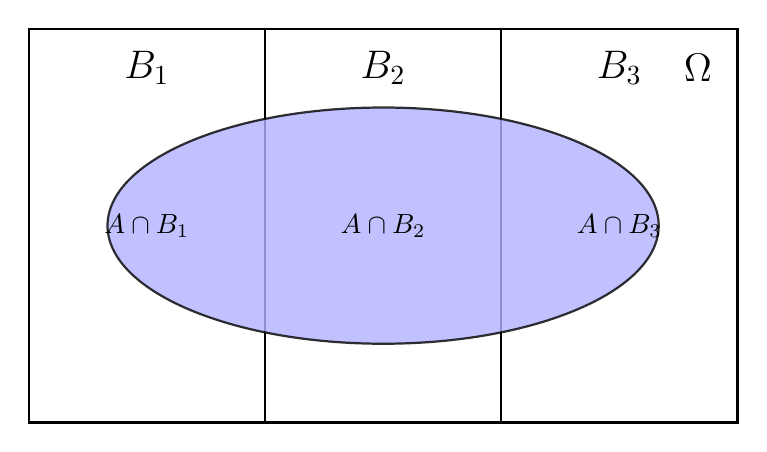
\begin{tikzpicture}
  % Draw sample space
  \draw[thick] (0,0) rectangle (9,5);
  \node at (8.5, 4.5) {\Large $\Omega$};
  
  % Draw partitions
  \draw[thick] (3,0) -- (3,5);
  \draw[thick] (6,0) -- (6,5);
  
  % Labels for partitions
  \node at (1.5, 4.5) {\Large $B_1$};
  \node at (4.5, 4.5) {\Large $B_2$};
  \node at (7.5, 4.5) {\Large $B_3$};
  
  % Draw event A (ellipse)
  \draw[thick, fill=blue!30, opacity=0.8] (4.5, 2.5) ellipse (3.5cm and 1.5cm);
  
  % Labels for Event A intersections
  \node at (1.5, 2.5) {$A \cap B_1$};
  \node at (4.5, 2.5) {$A \cap B_2$};
  \node at (7.5, 2.5) {$A \cap B_3$};
  
\end{tikzpicture}
\end{center}

\subsection{Heuristics \& "Cheats"}
\begin{itemize}
    \item \textbf{The "At Least One" Rule:} If a question asks for the probability of "at least one" event happening, immediately calculate $1 - \mathbb{P}(\text{none})$.
    \item \textbf{Independence vs. Mutually Exclusive:} These are opposites in most cases! If $A$ and $B$ are mutually exclusive (and have non-zero probability), they \textbf{cannot} be independent. If $A$ happens, $B$ definitely does not happen, meaning information about $A$ heavily influences $B$.
\end{itemize}

\subsection{Pitfalls \& Fallacies}
\begin{itemize}
    \item \textbf{The Base Rate Fallacy:} Ignoring $\mathbb{P}(B)$ when evaluating conditional probability $\mathbb{P}(A|B)$. (Common in false-positive medical testing).
    \item \textbf{Assuming Pairwise $\implies$ Mutual Independence:} Just because events $A, B$, and $C$ are independent in pairs does NOT mean $\mathbb{P}(A \cap B \cap C) = \mathbb{P}(A)\mathbb{P}(B)\mathbb{P}(C)$.
\end{itemize}

\newpage
% ==========================================
% PART 5: CONCEPTUAL SYNTHESIS
% ==========================================
\section{Part 5: Conceptual Synthesis and The "Big Picture"}

\subsection{A) Thematic Connections: The Measure-Theoretic Bridge}
This topic transitions students from \textit{counting} (discrete sample points) to \textit{measuring}. By treating probabilities as continuous algebraic objects, we decouple our logic from dice or cards. The core theme is \textbf{localization} (conditional probability) and \textbf{orthogonality} (independence). This mirrors linear algebra, where orthogonal vectors provide no information about each other, just as independent probabilistic events provide no information about one another's occurrence.

\subsection{B) Forward and Backward Links}
Backward, this builds directly on naive set theory and combinatorics, providing the necessary fractional weights to subset cardinality. Forward, understanding that conditional probability constitutes a valid probability space is the gateway to \textbf{Filtrations} and \textbf{Martingales}. In advanced Stochastic Calculus, conditional probability evolves into conditioning on an increasing field of information over time, denoted as $\mathbb{E}[X | \mathcal{F}_t]$, which is the backbone of modeling Brownian Motion.

% ==========================================
% PART 6: ABSTRACT REAL-WORLD MODELING
% ==========================================
\section{Part 6: Abstract Real-World Modeling (AI, ML, \& Quant Finance)}

\subsection{A) Concrete Scenarios}
\begin{enumerate}
    \item \textbf{Generative AI \& Bayesian Networks:} Large Language Models and expert systems operate on massive directed acyclic graphs of conditional probabilities. The network infers the hidden state of a system given observational evidence by repeatedly applying the multiplicative laws of probability.
    \item \textbf{Quantitative Finance \& Default Contagion:} In credit derivatives pricing, understanding if the default of Lehman Brothers (Event $A$) is independent of the default of AIG (Event $B$) is critical. Miscalculating $\mathbb{P}(A \cap B)$ by falsely assuming independence was the primary mathematical failure leading to the 2008 Financial Crisis.
\end{enumerate}

\subsection{B) Model Problem Setup: Credit Default Copulas}
We model default contagion in a portfolio of collateralized debt obligations (CDOs) using abstract conditional probability. 
\vspace{0.5em}

\textbf{Theoretical Framework:}
Let $(\Omega, \mathcal{F}, \mathbb{P})$ be our probability space. Consider two firms, 1 and 2. 
Let $\tau_1, \tau_2 \in [0, \infty)$ be continuous random variables representing the time to default for Firm 1 and Firm 2, respectively.
Let $D_1 = \{ \tau_1 \le T \}$ and $D_2 = \{ \tau_2 \le T \}$ be the events that Firm 1 and Firm 2 default before maturity time $T$.

In standard structural models, we assume marginal probabilities of default $\mathbb{P}(D_1) = p_1$ and $\mathbb{P}(D_2) = p_2$. If default risk were independent, the probability of joint default is trivial: $\mathbb{P}(D_1 \cap D_2) = p_1 p_2$. 

However, they are deeply dependent. We define a \textit{Gaussian Copula} dependency structure. We construct standard normal variables $X_1, X_2 \sim \mathcal{N}(0,1)$ such that the correlation between them is $\rho$. 
The events map to structural barriers:
\[ \mathbb{P}(D_1) = \mathbb{P}(X_1 \le \Phi^{-1}(p_1)) \quad \text{and} \quad \mathbb{P}(D_2) = \mathbb{P}(X_2 \le \Phi^{-1}(p_2)) \]
where $\Phi^{-1}$ is the inverse standard normal CDF. 

The \textbf{conditional probability of contagion}—the probability Firm 1 defaults \textit{given} Firm 2 defaults—is:
\[ \mathbb{P}(D_1 | D_2) = \frac{\mathbb{P}(D_1 \cap D_2)}{\mathbb{P}(D_2)} = \frac{\Phi_2(\Phi^{-1}(p_1), \Phi^{-1}(p_2); \rho)}{p_2} \]
where $\Phi_2$ is the bivariate normal CDF. By tuning the correlation parameter $\rho$, quantitative analysts construct the joint distribution. If $\rho = 0$, $\mathbb{P}(D_1 | D_2) = \mathbb{P}(D_1)$ (Independence). If $\rho \to 1$, default becomes virtually certain. Optimizing this joint measure to match empirical market spreads is a continuous nonlinear optimization problem deeply rooted in the foundational conditional axioms.

\newpage
% ==========================================
% PART 7: COMMON VARIATIONS & UNTESTED CONCEPTS
% ==========================================
\section{Part 7: Common Variations and Untested Concepts}

A standard advanced curriculum includes the concept of limits of infinite sets of events, specifically the \textbf{Borel-Cantelli Lemma}. The homework addresses infinite sequences of independent events (Problem 2.119), but ignores the measure-theoretic convergence of such sequences.

\begin{theorem}[First Borel-Cantelli Lemma]
Let $\{A_n\}_{n=1}^\infty$ be a sequence of events in a probability space. If the sum of their probabilities is finite:
\[ \sum_{n=1}^\infty \mathbb{P}(A_n) < \infty \]
then the probability that infinitely many of these events occur is zero. Notationally, $\mathbb{P}(\limsup_{n \to \infty} A_n) = 0$.
\end{theorem}

\begin{proof}[Proof of Untested Concept]
Let $E = \limsup_{n \to \infty} A_n = \bigcap_{N=1}^\infty \bigcup_{n=N}^\infty A_n$.
By definition, for any integer $N \ge 1$:
\[ E \subseteq \bigcup_{n=N}^\infty A_n \]
Using monotonicity of probability and subadditivity (Boole's Inequality):
\[ \mathbb{P}(E) \le \mathbb{P}\left( \bigcup_{n=N}^\infty A_n \right) \le \sum_{n=N}^\infty \mathbb{P}(A_n) \]
Because the infinite series $\sum_{n=1}^\infty \mathbb{P}(A_n)$ converges to a finite value, the tail of the series must approach 0 as $N \to \infty$:
\[ \lim_{N \to \infty} \sum_{n=N}^\infty \mathbb{P}(A_n) = 0 \]
Since $\mathbb{P}(E) \le 0$ and probability axioms require $\mathbb{P}(E) \ge 0$, we must conclude $\mathbb{P}(E) = 0$. $\blacksquare$
\end{proof}

\newpage
% ==========================================
% PART 8: ADVANCED DIAGNOSTIC TESTING
% ==========================================
\section{Part 8: Advanced Diagnostic Testing: "Find the Flaw"}

Below are five proofs that appear correct but contain a subtle mathematical fallacy. Your task is to act as the grader, identify the error, and provide the correct step. (The resolutions are in the Solution Key).

\subsection{Diagnostic Problems}

\textbf{Proof 1: "The Absolute Independence Paradox"} \\
\textit{Claim:} If $A$ and $B$ are mutually exclusive, and $A$ and $C$ are independent, then $B$ and $C$ must be dependent. \\
\textit{Provided Proof:} Since $A$ and $B$ are mutually exclusive, $A \cap B = \emptyset$. Since $A$ and $C$ are independent, $\mathbb{P}(A \cap C) = \mathbb{P}(A)\mathbb{P}(C)$. Suppose for contradiction $B$ and $C$ are independent, so $\mathbb{P}(B \cap C) = \mathbb{P}(B)\mathbb{P}(C)$. Combining these gives $\mathbb{P}((A \cup B) \cap C) = \mathbb{P}(A \cap C) + \mathbb{P}(B \cap C) = \mathbb{P}(C)[\mathbb{P}(A) + \mathbb{P}(B)]$. This limits the probability bounds. Thus, independence is violated. $\blacksquare$

\textbf{Proof 2: "The Universal Conditional Divider"} \\
\textit{Claim:} $\mathbb{P}(A | B \cup C) = \mathbb{P}(A | B) + \mathbb{P}(A | C)$. \\
\textit{Provided Proof:} We know that probability acts identically in conditional spaces. By the additive law, probabilities of unions expand. Thus, isolating $A$ relative to the union of $B$ and $C$ means we just add the conditional probabilities of $A$ given $B$ and $A$ given $C$. $\blacksquare$

\textbf{Proof 3: "Geometric Convergence Certainty"} \\
\textit{Claim:} In a sequential game, the probability of Event $A$ occurring eventually is 1, provided we have infinite time. \\
\textit{Provided Proof:} Let Event $A$ have probability $\mathbb{P}(A) = p$. Let Event $C$ be the failure, $\mathbb{P}(C) = (1+p)$. We evaluate the probability over infinite time as an infinite series: $\sum_{k=0}^\infty p (1+p)^k$. Using the formula $\frac{a}{1-r}$, we get $\frac{p}{1-(1+p)} = \frac{p}{-p} = -1$. Because probability cannot be negative, we take the absolute value, yielding 1. $\blacksquare$

\textbf{Proof 4: "Bayesian Reversal of Fortune"} \\
\textit{Claim:} If $\mathbb{P}(A|B) = \mathbb{P}(B|A)$, then $\mathbb{P}(A) = \mathbb{P}(B)$. \\
\textit{Provided Proof:} We begin with the assumption $\mathbb{P}(A|B) = \mathbb{P}(B|A)$. By definition, $\frac{\mathbb{P}(A \cap B)}{\mathbb{P}(B)} = \frac{\mathbb{P}(B \cap A)}{\mathbb{P}(A)}$. Since intersection is commutative, the numerators are identical. Therefore, we can cross-multiply to get $\mathbb{P}(A \cap B)\mathbb{P}(A) = \mathbb{P}(A \cap B)\mathbb{P}(B)$. Dividing both sides by $\mathbb{P}(A \cap B)$ yields $\mathbb{P}(A) = \mathbb{P}(B)$. $\blacksquare$

\textbf{Proof 5: "The Unbounded Bonferroni"} \\
\textit{Claim:} For any events $A, B, C$, $\mathbb{P}(A \cap B \cap C) \ge \mathbb{P}(A) + \mathbb{P}(B) + \mathbb{P}(C) - 1$. \\
\textit{Provided Proof:} We proved previously that $\mathbb{P}(A \cap B) \ge \mathbb{P}(A) + \mathbb{P}(B) - 1$. Let $X = A \cap B$. Substitute $X$ into the formula with $C$: $\mathbb{P}(X \cap C) \ge \mathbb{P}(X) + \mathbb{P}(C) - 1$. Substituting $X$ yields $\mathbb{P}(A \cap B \cap C) \ge \mathbb{P}(A \cap B) + \mathbb{P}(C) - 1$. We know $\mathbb{P}(A \cap B) \ge \mathbb{P}(A) + \mathbb{P}(B)$. Thus, $\mathbb{P}(A \cap B \cap C) \ge \mathbb{P}(A) + \mathbb{P}(B) + \mathbb{P}(C) - 1$. $\blacksquare$

\vspace{1em}
\hrule
\vspace{1em}

\subsection{Solution Key (Resolutions to Diagnostic Flaws)}
\begin{enumerate}
    \item \textbf{Flaw 1:} Circular and baseless algebraic leap. The equality $\mathbb{P}(C)[\mathbb{P}(A) + \mathbb{P}(B)]$ perfectly equals $\mathbb{P}((A \cup B) \cap C)$ if $B$ and $C$ are independent. There is no contradiction. To disprove the claim, simply set $C = \Omega$. Then $A$ and $C$ are independent, and $B$ and $C$ are independent, completely violating the claim.
    \item \textbf{Flaw 2:} Conditioning on a union does NOT linearly decompose. The correct formula is $\mathbb{P}(A | B \cup C) = \frac{\mathbb{P}(A \cap (B \cup C))}{\mathbb{P}(B \cup C)}$. You cannot arbitrarily split denominators in fractions.
    \item \textbf{Flaw 3:} The geometric series formula $S = \frac{a}{1-r}$ is strictly valid ONLY when $|r| < 1$. Here, the ratio $r = 1+p > 1$. The series diverges to infinity, and applying the formula yields absurd negative probabilities.
    \item \textbf{Flaw 4:} Division by zero! The proof divides both sides by $\mathbb{P}(A \cap B)$. If $A$ and $B$ are mutually exclusive, then $\mathbb{P}(A \cap B) = 0$, meaning the division is mathematically illegal. (The claim holds only if $\mathbb{P}(A \cap B) > 0$).
    \item \textbf{Flaw 5:} A substitution error in inequalities. The proof assumes $\mathbb{P}(A \cap B) \ge \mathbb{P}(A) + \mathbb{P}(B)$, which is profoundly false (that would mean intersections are larger than their parts). The correct Bonferroni lower bound substitution is $\mathbb{P}(A \cap B \cap C) \ge [\mathbb{P}(A) + \mathbb{P}(B) - 1] + \mathbb{P}(C) - 1 = \mathbb{P}(A) + \mathbb{P}(B) + \mathbb{P}(C) - 2$.
\end{enumerate}

\end{document}